\section{Method}

PrexSyn is a framework for synthesizable molecular design that introduces new contributions spanning model architecture, data infrastructure, and inference algorithms.
In this section, we will first describe the decoder-only transformer architecture of PrexSyn (Section~\ref{sec:method:model}), which unifies molecular properties and synthesizable molecular generation.
We then present the real-time, high-throughput data generation engine (Section~\ref{sec:method:data}), which plays the key role in scaling up training to billions of pathways under a modest compute budget.
Finally, we detail the inference-time algorithms for sampling molecules under multiple-property constraints expressed as logical queries (Section~\ref{sec:method:sampling}), and we show how this querying capability enables efficient molecular sampling against black-box oracles (Section~\ref{sec:method:optimization}), making PrexSyn a highly efficient general-purpose tool for molecular design.

\subsection{Decoder-only transformer architecture unifies property and synthesis}
\label{sec:method:model}
PrexSyn is based on a decoder-only transformer \citep{vaswani2017attention} which takes as input a prompt of molecular properties and then autoregressively generates postfix notations of synthesis (Figure~\ref{fig:network}b).
Formally, the model learns the following conditional distribution:
\begin{equation}
    p (\vs | \mC) = \prod_{i=1}^{N} p(s_i | s_{<i}, \mC).
\end{equation}
Here, $\mC$ is the property prompt generated by embedding property values with simple linear layers.
$\vs = [s_1, \ldots, s_N]$ is the tokenized postfix notation sequence, where each building block and each reaction corresponds to a unique token associated with a learnable embedding vector.
Positional encodings are added to the token embeddings to indicate the order \citep{vaswani2017attention}.
To predict the next token, the model adopts a two-level approach. First, it predicts the type of the next token (\textit{i.e.}, building block, reaction, \texttt{[START]}, or \texttt{[END]}). If the predicted type is a building block or reaction token, a second-level classifier is used to predict the specific token within that class.
This two-level classifier is similar to the routing mechanism in mixture-of-expert models \citep{eigen2013learning}, as it avoids retrieving building blocks at every step.
Formally, the conditional distribution of the next token is given by:
\begin{equation}
    p(s_i | s_{<i}, \mC) = \begin{cases}
        p\left(T(s_i) = \texttt{BB} \mid \cdots \right) p\left(s_i \mid T(s_i) = \texttt{BB}, \cdots \right)  & T(s_i) = \texttt{BB} \\
        p\left(T(s_i) = \texttt{RXN} \mid \cdots \right) p\left(s_i \mid T(s_i) = \texttt{RXN}, \cdots \right)  & T(s_i) = \texttt{RXN} \\
        p\left(s_i \mid \cdots \right)  & \text{otherwise}
    \end{cases},
\end{equation}
where $T(s_i)$ denotes the type of the token $s_i$.

The transformer is trained using standard cross-entropy loss with causal masking to maximize the likelihood of the postfix notation sequence conditioned on their property prompts.
At inference time, to generate molecules conditioned on a single property prompt, we first embed the prompt and prepend the embedding vectors to the \texttt{[START]} token.
Then, we autoregressively sample tokens until the \texttt{[END]} token is emitted.

Note that we use a classifier to select building blocks from the library, with each class corresponding to a specific building block.
This differs from previous models, which rely on molecular fingerprints to retrieve building blocks via deterministic nearest-neighbor retrievial \citep{luo2024projecting}.
Fingerprint-based selection is limited to structural similarity and is not adaptable to varying contexts.
In contrast, the classifier-based approach allows dynamic selection of building blocks based on the context provided by property prompts through the learnable unembedding matrix.
In addition, it naturally allows probabilistic sampling from the building block library, which is crucial for generating diverse synthetic pathways in the property-conditioned setting as there is no one-to-one relationship between properties and molecules.

While direct tokenization of building blocks leads to the introduction of a large number of distinct tokens, the computational overhead is manageable at training time and negligible at inference time.
The number of in-stock building blocks offered by commercial vendors today typically does not exceed one million.
For example, as of November 2025, Enamine lists about 480 thousand building blocks in its global stock \citep{enamineBuildingBlocks} and WuXi lists about 90 thousand \citep{wuxi}.
With an embedding dimension of 1,024 and 32-bit floating-point precision, the combined memory cost of the embedding and unembedding matrices for 1 million building blocks is $2 \times 10^{6} \times 1,024 \times 4 \text{ bytes} \approx 8 \text{ GB}$, which is affordable on modern GPUs.
If we reduce the floating point precision to 16-bit, the memory cost will be halved.
At inference time, the embedding matrix does not need to be loaded into GPU memory, since only a small number of building block embeddings are looked up.
Moreover, the unembedding matrix does not introduce significant inference-time memory overhead compared with fingerprint-based models \citep{luo2024projecting,gao2025generative}, which store the all building block fingerprints in GPU memory for nearest-neighbor retrieval.
Even if the number of in-stock building blocks grows drastically in the future, we can still use techniques such as sampled softmax \citep{blanc2018adaptive} and cut cross-entropy \citep{wijmans2024cut} to keep the memory and computation bounded.


Another challenge with building block tokenization is that the embeddings are initialized randomly without any prior, which requires more training data than fingerprint-based representations encoding structural prior about building block.
However, as we will describe in the next section, our high-throughput training data generation engine makes billion-scale training data feasible under moderate compute budget, thereby providing sufficient data for the model to learn meaningful building block embeddings from scratch.


\begin{figure}[t]
\begin{center}
\centerline{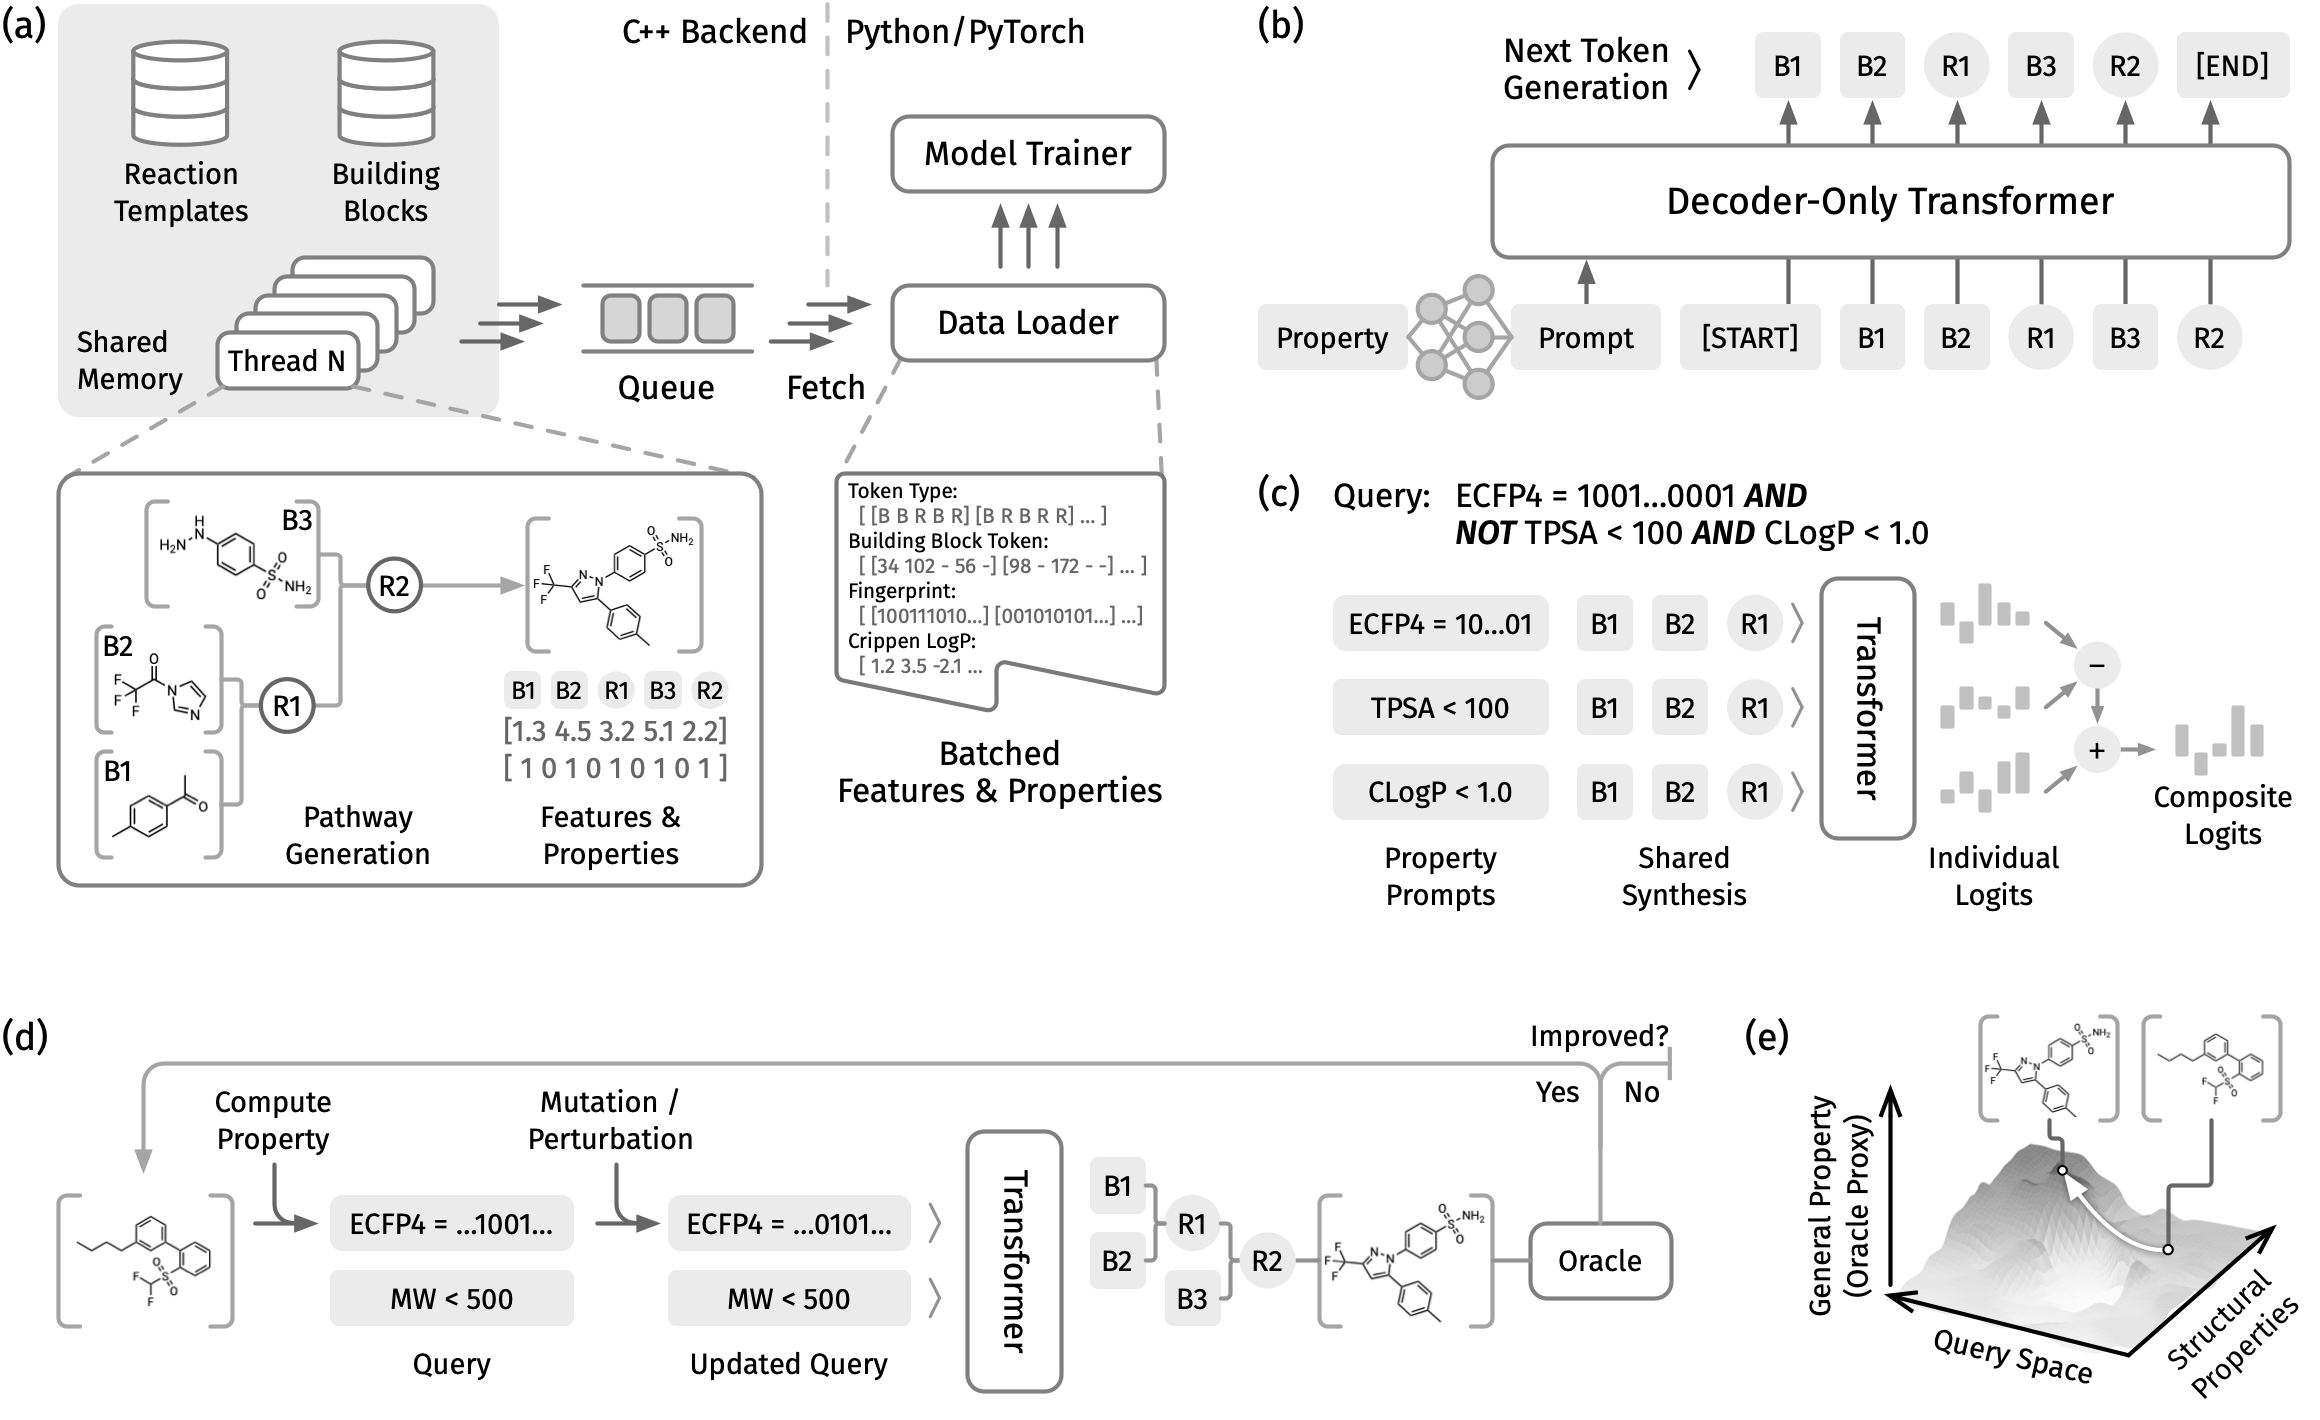
\includegraphics[width=\linewidth]{figures/fig1.png}}
\vspace{0.5em}
\caption{
  \textbf{(a)} The high-throughput C\texttt{++} data engine generates synthetic pathways and computes molecular properties on the fly. It adopts a producer-consumer architecture, where multiple producer threads generate and featurize samples, which are then consumed by the Python-based training framework.
  \textbf{(b)} The decoder-only transformer architecture predicts the next token conditioned on property prompts.
  \textbf{(c)} Multiple properties in a composite query are used to condition the model separately. The resulting distributions are then combined.
  \textbf{(d)} Query space optimization. At each step, molecular properties are computed and perturbed to recondition the model. New molecules are then evaluated by oracle functions, and those with improved properties replace previous ones.
  \textbf{(e)} Since the structural properties used for training are sufficiently expressive to locate molecules, we can sample molecules with respect to general properties defined by black-box oracles by iteratively refining structural-property queries.
}
\label{fig:network}
\end{center}
\end{figure}


\subsection{High-throughput data engine enables billion-scale training datastream}
\label{sec:method:data}

Training data are generated on the fly by randomly sampling synthetic pathways from the combinatorial space defined by the building block library and reaction template set, paired with their molecular properties.
This real-time approach enables virtually unlimited training data that scales with training time.
However, its efficiency is limited in Python implementations \citep{luo2024projecting} due to the lack of thread-level parallelism and the overhead of function calls through Python bindings, resulting in a bottleneck in training throughput given the highly optimized standard transformer architecture used.

To overcome this bottleneck, we developed a  multi-threaded data pipeline in C\texttt{++} that generates synthetic pathways and computes molecular properties using the RDKit C\texttt{++} API \citep{rdkit}.
It adopts a producer-consumer architecture (Figure~\ref{fig:network}a): multiple producer threads generate synthetic pathways, compute molecular properties, and featurize them into tensors, which are pushed into a queue buffer.
The data loader of the training framework, which acts as the consumer, fetches featurized batches from the buffer, transfers them to GPU memory, and feeds them into the model for training.

The C\texttt{++}-based pipeline achieves a throughput of over 6,000 samples per second on 32 threads (16 cores) benchmarked on an AMD Ryzen Threadripper PRO 5975WX CPU, providing abundant throughput for training our transformer-based model on NVIDIA H100 GPUs.
Another noteworthy advantage of our implementation is its low memory cost benefits from the shared memory space. It allows scaling up the number of threads without a significant increase in memory usage, whereas the previous Python-based implementation's memory cost grows linearly with the number of processes as each process requires a copy of the building block library.
The model used for evaluation in this work was trained on two NVIDIA H100 GPUs with 32 CPU cores for 640,000 steps over 48 hours, using a batch size of 2,048 per step, resulting in a total of about 1.3 billion training pathways.


We also implemented a multi-threaded C\texttt{++} function for batched detokenization at inference time.
It takes as input a batch of postfix notation tokens, distributes the sequences to multiple threads, converts them into synthetic pathways, and obtains the product molecules with RDKit.


\subsection{Training setup}
\label{sec:method:training}

Following previous works \citep{luo2024projecting,gao2025generative,lee2025rethinking}, we used Enamine US in-stock building block set retrieved on October 1, 2023 and the reaction template set curated by \cite{gao2025generative} which contains 115 reaction templates. 

The model consists of 12 transformer layers, with a model dimension of 1,024, a feedforward dimension of 2,048, and 16 attention heads. Excluding the embedding and unembedding matrices for building blocks, the transformer backbone together with other embedding layers has about 131 million parameters.
When including these matrices, the total number of trainable parameters increases to 589 million.
The model is optimized using the Adam optimizer with an initial learning rate of $3\times 10^{-4}$ and a batch size of 2,048. A cosine annealing learning rate scheduler is used with $T_\text{max}=500$ and $\eta_\text{min}=10^{-5}$. The scheduler is triggered after each validation epoch.
Validation is conducted every 2,000 training steps on random synthetic pathways.
The model is trained using 32-bit full-precision floating point, with no mixed-precision or low-precision optimizations. Training runs for 48 hours on two NVIDIA H100 GPUs, corresponding to 640,000 iterations.

We train the model using the following structural properties widely used in quantitative structure-activity relationship (QSAR) studies \citep{roy2015qsarbook}:
(1) ECFP4 fingerprint \citep{rogers2010extended};
(2) Gobbi pharmacophoric feature-based FCFP4 fingerprint \citep{gobbi1998genetic};
(3) BRICS decomposition-based substructures \citep{degen2008art}; and
(4) physicochemical descriptors from RDKit including molecular weight, CLogP, TPSA, \textit{etc} \citep{rdkit}.

Each training sample consists of only one property type randomly selected from the properties above paired with a synthetic pathway.


\subsection{Generating molecules according to composite property queries}
\label{sec:method:sampling}

As the model is trained using pairs consisting of a single property and a synthetic pathway, it does not learn the distribution of molecules conditioned on multiple properties, which is often required in practical scenarios.
A naive solution would be to include multiple properties in every training sample, but the amount of data required for training in this way grows exponentially with the number of property types \citep{du2024position}.
To avoid this bottleneck, we formulate a method to compose multiple properties at inference time.
First, consider two different property prompts: $\mC_1$ and $\mC_2$; $p(\vs | \mC_1)$ and $p(\vs | \mC_2)$ are the distributions of postfix notations conditioned on each prompt respectively.

\paragraph{AND (Conjunction)}
The conditional distributions for molecules satisfying both conditions $\mC_1$ and $\mC_2$ is the product of the two distributions:
\begin{equation}
\label{eq:and}
    p(\vs | \mC_1 \land \mC_2) \propto p(\vs | \mC_1)^\alpha  p(\vs | \mC_2)^\beta = \prod_{i=1}^{N}  p(s_i | s_{<i}, \mC_1)^\alpha  p(s_i | s_{<i}, \mC_2)^\beta \quad (\alpha, \beta > 0),
\end{equation}
where $\alpha$ and $\beta$ are hyperparameters that control the relative importance of each condition.
At each sampling step, we first compute the conditional distributions of the next token given each property prompt, and then combine them using the above equation to get the final distribution for sampling. Specifically, the combined distribution is given by:
\begin{equation}
\label{eq:and_logits}
    p(s_i | s_{<i}, \mC_1)^\alpha  p(s_i | s_{<i}, \mC_2)^\beta = \operatorname{softmax}\left( \alpha \vz_1 + \beta \vz_2 \right),
\end{equation}
where $\vz_1$ and $\vz_2$ are the logits of the next token predicted by the model given property prompts $\mC_1$ and $\mC_2$ respectively.

\paragraph{NOT (Negation)}
Similarly, the conditional distribution for molecules satisfying $\mC_1$ but not $\mC_2$ is given by:
\begin{equation}
\label{eq:not}
    p(\vs | \mC_1 \lnot \mC_2) \propto \frac{p(\vs | \mC_1)^\alpha}{p(\vs | \mC_2)^\beta} = \prod_{i=1}^{N}  \frac{p(s_i | s_{<i}, \mC_1)^\alpha}{p(s_i | s_{<i}, \mC_2)^\beta} \quad (\alpha, \beta > 0).
\end{equation}
The combined distribution for each sampling step is given by:
\begin{equation}
\label{eq:not_logits}
    p(s_i | s_{<i}, \mC_1 \lnot \mC_2) \propto \frac{p(s_i | s_{<i}, \mC_1)^\alpha}{p(s_i | s_{<i}, \mC_2)^\beta} = \operatorname{softmax}\left( \alpha \vz_1 - \beta \vz_2 \right).
\end{equation}

Note that the negation operation can be unified with the conjunction operation by allowing $\beta$ in equation \ref{eq:and} to take negative values, which provides a convenient formulation for implementation.

\paragraph{OR (Disjunction)}
Under the disjunction of two conditions $\mC_1$ and $\mC_2$, the distribution of molecules satisfying either condition is given by:
\begin{equation}
    p(\vs | \mC_1 \lor \mC_2) \propto \alpha p(\vs | \mC_1) + \beta p(\vs | \mC_2) = \alpha \prod_{i=1}^{N} p(s_i | s_{<i}, \mC_1)
    + \beta \prod_{i=1}^{N} p(s_i | s_{<i}, \mC_2).
\end{equation}
Unlike the previous two cases, this distribution cannot be factorized autoregressively. Therefore, we sample full sequences from each conditional distribution separately and then merge the samples to obtain the final set of molecules.

\paragraph{Composite logical queries}
We define \textit{query} ($\mQ$) as a logical expression over molecular properties composed using the logical operators AND, NOT, and OR.
To enable sampling from composite logical queries involving multiple properties connected by logical operators, we first convert the query into disjunctive normal form (DNF) \citep{rosen2019discrete}, \textit{i.e.} a series of ORs where each term only contains ANDs and NOTs.
For each conjunctive term, we apply equations \ref{eq:and_logits} and \ref{eq:not_logits} to get its composed distribution, from which samples are drawn.
Finally, we merge the samples from all conjunctive terms to obtain the final set of molecules satisfying the composite logical query.

The theoretical assumption underlies the above formulation is that property prompts are mutually conditionally independent given the molecule, and that the prior distribution over molecules is uniform.
Under these assumptions, the joint conditional distribution can be expressed in a product-of-experts form as shown in equations \ref{eq:and} and \ref{eq:not} \citep{hinton1999poe}.
Although some structural properties may be independent, many molecular properties are correlated, particularly those related to size such as molecular weight and number of rotatable bonds.
Nevertheless, this simplifying assumption is what allows us to derive a practical algorithm for composing multiple properties.
In practice, this assumption becomes problematic when there are contradictions among properties, such as simultaneously requiring molecular weight below 100 and number of heavy atoms above 50, which we consider detectable and avoidable in general.


\subsection{Synthesizable molecule sampling in query space}
\label{sec:method:optimization}


Although the properties used for training already span a broad range of structural and physicochemical characteristics that are frequently used in cheminformatics workflows, they do not cover the full space of molecular properties.
We need a mechanism to sample molecules with respect to properties that are not included during training, such as docking scores \citep{autodockgpu}, antibiotic activity \citep{stokes2020deep}, and so on.
A straightforward way is to fine-tune the model on the new properties, but this is inefficient and might require a large amount of property evaluations for training.

Fortunately, the property-based querying capability of PrexSyn opens a new avenue for sampling molecules with respect to general properties.
As the structural properties used for training are sufficiently expressive to locate molecules within the synthesizable chemical space, we can optimize molecules with respect to black-box oracle functions by iteratively refining property queries until satisfactory candidates are found (Figure~\ref{fig:network}e).
This makes PrexSyn a general-purpose tool for synthesizable molecular design.


The sampling process (Figure~\ref{fig:network}d) begins with a seed query $\mQ_0$, which is used to generate an initial set of candidate molecules.
At each iteration, each candidate molecule $\gM$ is mapped to a property query $\mQ_t$. In general, the property query takes the form
$\mQ = \mC^\text{(opt)}_1(\gM) \land \mC^\text{(opt)}_2(\gM) \land \cdots \mC^\text{(cstr)}_1 \land \cdots$,
where $\{ \mC^\text{(opt)}_i(\gM) \}$ denotes optimizable conditions dependent on $\gM$ and $\{ \mC^\text{(cstr)}_i \}$ denotes fixed constraints.
Next, perturbation is added to the optimizable term, resulting in an updated query
$\mQ' = {\mC'}^\text{(opt)}_1 \land \cdots \mC^\text{(cstr)}_1 \land \cdots$.
The updated query is then used to generate new candidate molecules, which are evaluated by the oracle.
New candidates that achieve a better oracle score will replace the old candidates, leading to an improved set of molecules.
Note that this process is described generically, and it may be implemented using genetic algorithms, Metropolis-Hastings sampling, or other iterative sampling methods. These implementations differ in how property queries are updated and how new candidates are selected.
